\documentclass[a4paper,10pt,landscape]{article}
\usepackage[margin=0.6cm]{geometry}
\usepackage[T1]{fontenc}
\usepackage[utf8]{inputenc}
\usepackage{xcolor}
\usepackage{tikz}
\usetikzlibrary{arrows.meta,positioning,calc,shapes.geometric}
\pagestyle{empty}
\setlength{\parindent}{0pt}
\renewcommand{\familydefault}{\sfdefault}

\definecolor{zw}{RGB}{0,0,0}
\definecolor{bl}{RGB}{20,70,180}
\definecolor{gr}{RGB}{20,120,40}
\definecolor{ro}{RGB}{180,20,20}

\newcommand{\ZW}[1]{\textcolor{zw}{#1}}
\newcommand{\BL}[1]{\textcolor{bl}{#1}}
\newcommand{\GR}[1]{\textcolor{gr}{#1}}
\newcommand{\RO}[1]{\textcolor{ro}{#1}}

\begin{document}

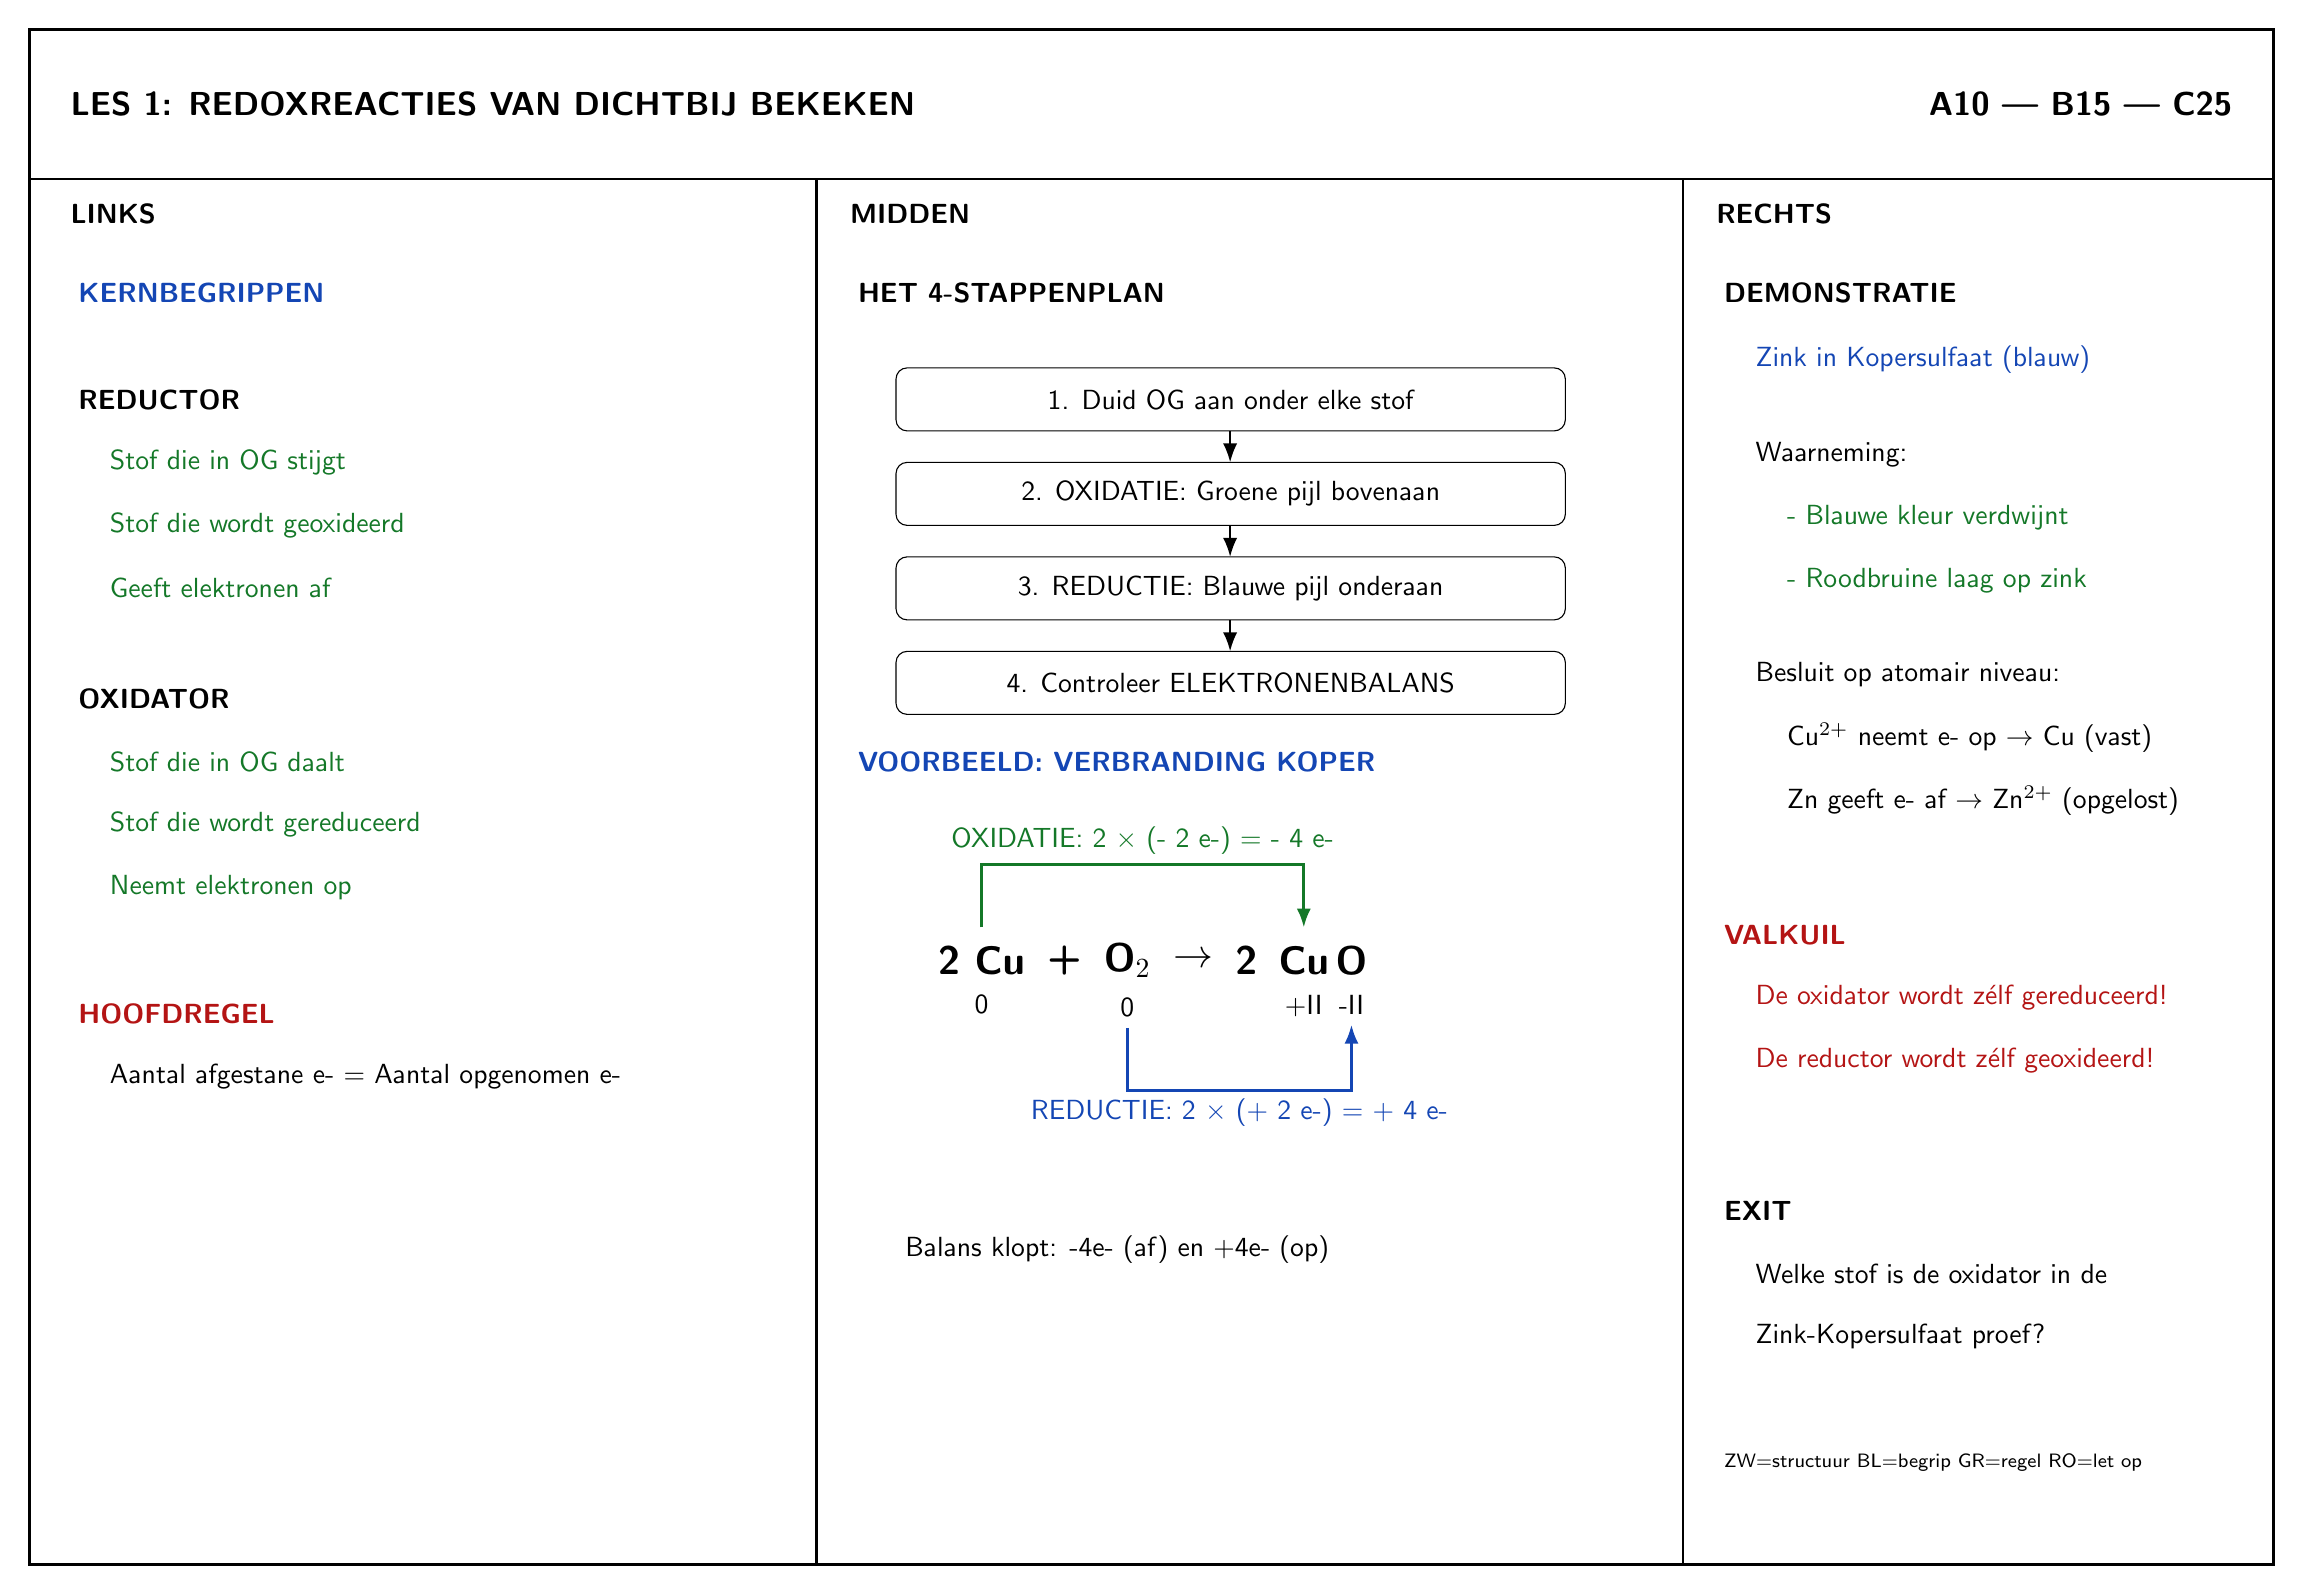
\begin{tikzpicture}[x=1cm,y=1cm]
  % outer board
  \draw[line width=1.2pt] (0,0) rectangle (28.5,19.5);

  % top bar
  \draw[line width=0.9pt] (0,17.6) -- (28.5,17.6);
  \node[anchor=west,font=\bfseries\large] at (0.4,18.55) {\ZW{LES 1: REDOXREACTIES VAN DICHTBIJ BEKEKEN}};
  \node[anchor=east,font=\bfseries\large] at (28.1,18.55) {\ZW{A10 | B15 | C25}};

  % vertical columns
  \draw[line width=0.9pt] (10.0,0) -- (10.0,17.6);
  \draw[line width=0.9pt] (21.0,0) -- (21.0,17.6);

  % column titles
  \node[anchor=west,font=\bfseries] at (0.4,17.15) {\ZW{LINKS}};
  \node[anchor=west,font=\bfseries] at (10.3,17.15) {\ZW{MIDDEN}};
  \node[anchor=west,font=\bfseries] at (21.3,17.15) {\ZW{RECHTS}};

  % left column (Concepts)
  \node[anchor=west,font=\bfseries] at (0.5,16.15) {\BL{KERNBEGRIPPEN}};
  
  \node[anchor=west,font=\bfseries] at (0.5,14.8) {\ZW{REDUCTOR}};
  \node[anchor=west] at (0.9,14.0) {\GR{Stof die in OG stijgt}};
  \node[anchor=west] at (0.9,13.2) {\GR{Stof die wordt geoxideerd}};
  \node[anchor=west] at (0.9,12.4) {\GR{Geeft elektronen af}};

  \node[anchor=west,font=\bfseries] at (0.5,11.0) {\ZW{OXIDATOR}};
  \node[anchor=west] at (0.9,10.2) {\GR{Stof die in OG daalt}};
  \node[anchor=west] at (0.9,9.4) {\GR{Stof die wordt gereduceerd}};
  \node[anchor=west] at (0.9,8.6) {\GR{Neemt elektronen op}};

  \node[anchor=west,font=\bfseries] at (0.5,7.0) {\RO{HOOFDREGEL}};
  \node[anchor=west] at (0.9,6.2) {\ZW{Aantal afgestane e- = Aantal opgenomen e-}};

  % middle column (Flowchart and Equation)
  \node[anchor=west,font=\bfseries] at (10.4,16.15) {\ZW{HET 4-STAPPENPLAN}};
  
  \node[draw,rounded corners,minimum width=8.5cm,minimum height=0.8cm,anchor=west] at (11.0,14.8) {\ZW{1. Duid OG aan onder elke stof}};
  \node[draw,rounded corners,minimum width=8.5cm,minimum height=0.8cm,anchor=west] at (11.0,13.6) {\ZW{2. OXIDATIE: Groene pijl bovenaan}};
  \node[draw,rounded corners,minimum width=8.5cm,minimum height=0.8cm,anchor=west] at (11.0,12.4) {\ZW{3. REDUCTIE: Blauwe pijl onderaan}};
  \node[draw,rounded corners,minimum width=8.5cm,minimum height=0.8cm,anchor=west] at (11.0,11.2) {\ZW{4. Controleer ELEKTRONENBALANS}};

  \draw[-{Latex[length=2.4mm]},line width=0.8pt] (15.25,14.4) -- (15.25,14.0);
  \draw[-{Latex[length=2.4mm]},line width=0.8pt] (15.25,13.2) -- (15.25,12.8);
  \draw[-{Latex[length=2.4mm]},line width=0.8pt] (15.25,12.0) -- (15.25,11.6);

  \node[anchor=west,font=\bfseries] at (10.4,10.2) {\BL{VOORBEELD: VERBRANDING KOPER}};
  
  \node[anchor=base west,font=\Large\bfseries,inner sep=1pt] (cuL) at (11.5,7.5) {\ZW{2 Cu}};
  \node[anchor=base west,font=\Large\bfseries,inner sep=1pt] (plus) [right=0.2cm of cuL] {\ZW{+}};
  \node[anchor=base west,font=\Large\bfseries,inner sep=1pt] (o2) [right=0.2cm of plus] {\ZW{O$_2$}};
  \node[anchor=base west,font=\Large\bfseries,inner sep=1pt] (arrow) [right=0.2cm of o2] {\ZW{$\rightarrow$}};
  \node[anchor=base west,font=\Large\bfseries,inner sep=1pt] (two) [right=0.2cm of arrow] {\ZW{2 }};
  \node[anchor=base west,font=\Large\bfseries,inner sep=1pt] (cuR) [right=0cm of two] {\ZW{Cu}};
  \node[anchor=base west,font=\Large\bfseries,inner sep=1pt] (oR) [right=0cm of cuR] {\ZW{O}};

  \node[anchor=north] at ([yshift=-0.1cm]cuL.south) {\ZW{0}};
  \node[anchor=north] at ([yshift=-0.1cm]o2.south) {\ZW{0}};
  \node[anchor=north] at ([yshift=-0.1cm]cuR.south) {\ZW{+II}};
  \node[anchor=north] at ([yshift=-0.1cm]oR.south) {\ZW{-II}};

  \draw[-{Latex[length=2.4mm]},line width=1.0pt,gr] ([yshift=0.2cm]cuL.north) -- ++(0,0.8) -| ([yshift=0.2cm]cuR.north);
  \node[anchor=south] at ($(cuL.north)!0.5!(cuR.north) + (0,1.0)$) {\GR{OXIDATIE: 2 $\times$ (- 2 e-) = - 4 e-}};

  \draw[-{Latex[length=2.4mm]},line width=1.0pt,bl] ([yshift=-0.6cm]o2.south) -- ++(0,-0.8) -| ([yshift=-0.6cm]oR.south);
  \node[anchor=north] at ($(o2.south)!0.5!(oR.south) + (0,-1.4)$) {\BL{REDUCTIE: 2 $\times$ (+ 2 e-) = + 4 e-}};

  \node[anchor=west] at (11.0,4.0) {\ZW{Balans klopt: -4e- (af) en +4e- (op)}};

  % right column (Demonstration and Pitfalls)
  \node[anchor=west,font=\bfseries] at (21.4,16.15) {\ZW{DEMONSTRATIE}};
  \node[anchor=west] at (21.8,15.3) {\BL{Zink in Kopersulfaat (blauw)}};
  
  \node[anchor=west] at (21.8,14.1) {\ZW{Waarneming:}};
  \node[anchor=west] at (22.2,13.3) {\GR{- Blauwe kleur verdwijnt}};
  \node[anchor=west] at (22.2,12.5) {\GR{- Roodbruine laag op zink}};

  \node[anchor=west] at (21.8,11.3) {\ZW{Besluit op atomair niveau:}};
  \node[anchor=west] at (22.2,10.5) {\ZW{Cu$^{2+}$ neemt e- op $\rightarrow$ Cu (vast)}};
  \node[anchor=west] at (22.2,9.7) {\ZW{Zn geeft e- af $\rightarrow$ Zn$^{2+}$ (opgelost)}};

  \node[anchor=west,font=\bfseries] at (21.4,8.0) {\RO{VALKUIL}};
  \node[anchor=west] at (21.8,7.2) {\RO{De oxidator wordt zélf gereduceerd!}};
  \node[anchor=west] at (21.8,6.4) {\RO{De reductor wordt zélf geoxideerd!}};

  \node[anchor=west,font=\bfseries] at (21.4,4.5) {\ZW{EXIT}};
  \node[anchor=west] at (21.8,3.7) {\ZW{Welke stof is de oxidator in de}};
  \node[anchor=west] at (21.8,2.9) {\ZW{Zink-Kopersulfaat proef?}};

  \node[anchor=west,font=\scriptsize] at (21.4,1.3) {\ZW{ZW=structuur  BL=begrip  GR=regel  RO=let op}};
\end{tikzpicture}

\end{document}
